\chapter{Система имитационного моделирования.}

\section{Интерфейс имитационного моделирования}

\subsection{Входные данные}
Некоторые из приведенных данных не учтены в текущей реализации, планируется добавление их в будущем. Эти данные \textit{помечены таким образом}.

\begin{itemize}
	\item ЦПВ - цеховая последовательность выпуска (выпуск продукции осуществляется в порядке, в котором они записаны в ЦПВ):
		\begin{itemize}
			\item наименование продукции;
			\item количество единиц продукции;	
			\item технологическая карта.
		\end{itemize}			
	\item Технологические карты, подробнее смотри (\ref{assembly_line_balancing:input_data}).
	\item Производственные ресурсы;
	\item \textit{Трафик доступности ресурсов};
	\item \textit{Структура цеха};
	\item \textit{Минимальное время участия ресурса в операции};
	\item \textit{Штрафы за переключение ресурса с одной операции на другую}. 
\end{itemize}

\subsection{Выходные данные}

\begin{itemize}
	\item Расчетные данные:	
		\begin{itemize}
			\item Перечень всех операций для всех единиц продукции ЦПВ;
			\item Время начала всех операций;
			\item Время окончания всех операций;
			\item \textit{Производственные ресурсы, привлекаемые к выполнению операции};
			\item \textit{Время начала и конца участия ресурса в операции};
			\item \textit{Загрузка производственных ресурсов}.
		\end{itemize}		
	\item Визуализиация данных пользователю:
		\begin{itemize}
			\item Расписания для производственных ресурсов;
			\item Диаграммы Ганта выпуска разных видов продукции;
			\item Визуализация загрузки производственных ресурсов.
		\end{itemize}		 
\end{itemize}

\section{Предобработка технологических карт}

input:

output:

Одним из первых этапов работы алгоритма имитационного моделирования является подготовка входных данных. Входными данными имитационного моделирования являются: технологические карты, состав заказа, ресурсы предприятия, а также другие конфигурации.

На текущий момент реализована небольшая часть функционала отвечающую за предварительную обработку. Одной из таких функций является расчет длительности операций. Так как длительность операций является переменной величиной, зависимой от трудоемкости и количества людей выполняющих операцию, существует 4 настройки ресурса:

\begin{itemize}
    \item минимальная, при этом на операцию назначается минимальное количество людей, отсюда и длительность операции становится максимальной
    \item максимальная
    \item средняя
    \item случайная, данная конфигурация является частью работы эвристических алгоритмов, рассматриваемых в следующей главе
\end{itemize}

Также одной из возможностей предварительной настройки является алгоритм выбора операций последовательности(в тех случаях, когда позволяет причинно-следственная часть). На данный момент существует 2 конфигурации:

\begin{itemize}
    \item стандартная, при которой выбор осуществляется строго по порядку расположения в структурах данных
    \item случайная, при этом случайным образом выбирается одна из возможных операций, которые доступны в данный момент 
\end{itemize}

Возможность менять входные данные являются важным этапом обработки входных данных полученных из базы данных, позволяя при этом подготовить данные для дальнейшей обработки, а также гибко менять параметризуемые величины, чем и достигается большая вариативность, так необходимая для поиска оптимального значения. 

\section{Создание шаблона плана}


input:

output:

\section{Имитационное планирование}

input:

output:

\section{Оптимизация средствами имитацонного моделирования}

\subsubsection{Метод полного перебора}
Примером оптимизации может служить случайный выбор следующей операции при планировании, данный выбор возможен только в случаях одновременного выполнения нескольких независимых операций. Таким образом достигается вариативность при котором из разных реализаций, выбирается наилучший вариант. На рисунке (\ref{ris:Force}) изображены технологическая карта продукта и два плана, который были построены в результате случайного выбора операций. Как видно из рисунка (\ref{ris:Force}) первый план является более оптимальным по времени и ресурсам, чем второй.

\begin{figure}[H]
    \center{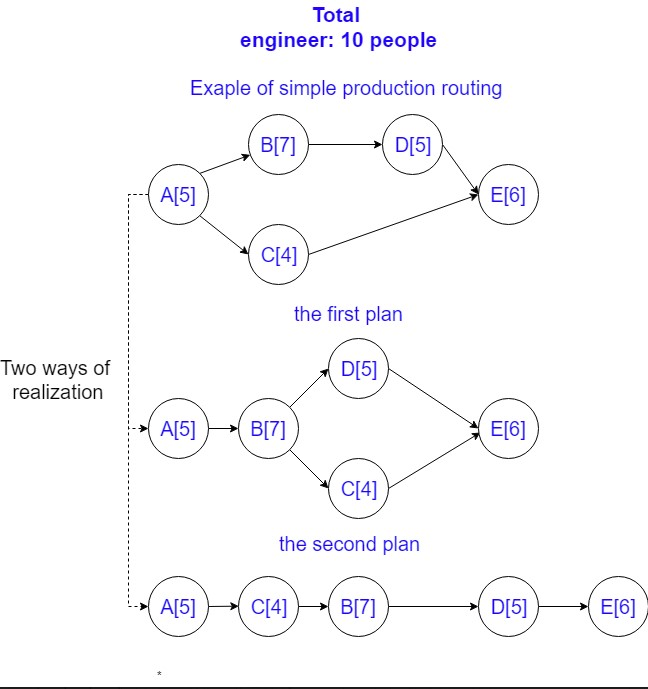
\includegraphics[width=1\linewidth]{fig/Force.jpg}}
    \caption{Два плана, полученные путем перебора исходной технологической карты}
    \label{ris:Force}
\end{figure}

\subsection{Методы оптимизации полного перебора}

\section{Результаты работы имитационной модели}